\documentclass{article}
 \usepackage{array}
\usepackage[utf8]{inputenc}
\usepackage[english]{babel}
\usepackage[document]{ragged2e}
\usepackage{amsfonts}
\usepackage{geometry}
\usepackage{amsmath,amssymb}


 \geometry{
 a4paper,
 total={170mm,257mm},
 left=10mm,
 top=20mm,
 }
\usepackage{lscape}
\usepackage{graphicx}
\usepackage{placeins}
\usepackage{float}
\usepackage{subfigure}
\newenvironment{psmallmatrix}
  {\left(\begin{smallmatrix}}
  {\end{smallmatrix}\right)}




\newcommand{\twopartdef}[4]
{
	\left\{
		\begin{array}{ll}
			#1 &  #2 \\
			#3 &  #4
		\end{array}
	\right.
}



\begin{document}
\justify
\section{Nonlinear VCO response dynamics, 3rd generation prototype}

Here we study a network of two mutually coupled $3rd$ generation PLLs taking into account the nonlinearity of the VCO's frequency response to the input control signal. 
%
The funtion we use is
%
\begin{equation} \label{N_delay_coupled}
	f\left( x^c(t) \right)=2\pi(a^\textrm{\tiny VCO}+b^\textrm{\tiny VCO}\,k\,\sqrt{V_{bias}+ x^c(t) } )
\end{equation}
where $x^c(t)$ the control signal, $a^\textrm{\tiny VCO}$ and $b^\textrm{\tiny VCO}$ are constant parameters which depend on the architecture and hence the nonlinearities of the VCO.
%
%Note, that here $a^\textrm{\tiny VCO}$ and $b^\textrm{\tiny VCO}$ are not the parameters of the architecture of the VCO. 

\begin{figure}[!h]
	\centering
	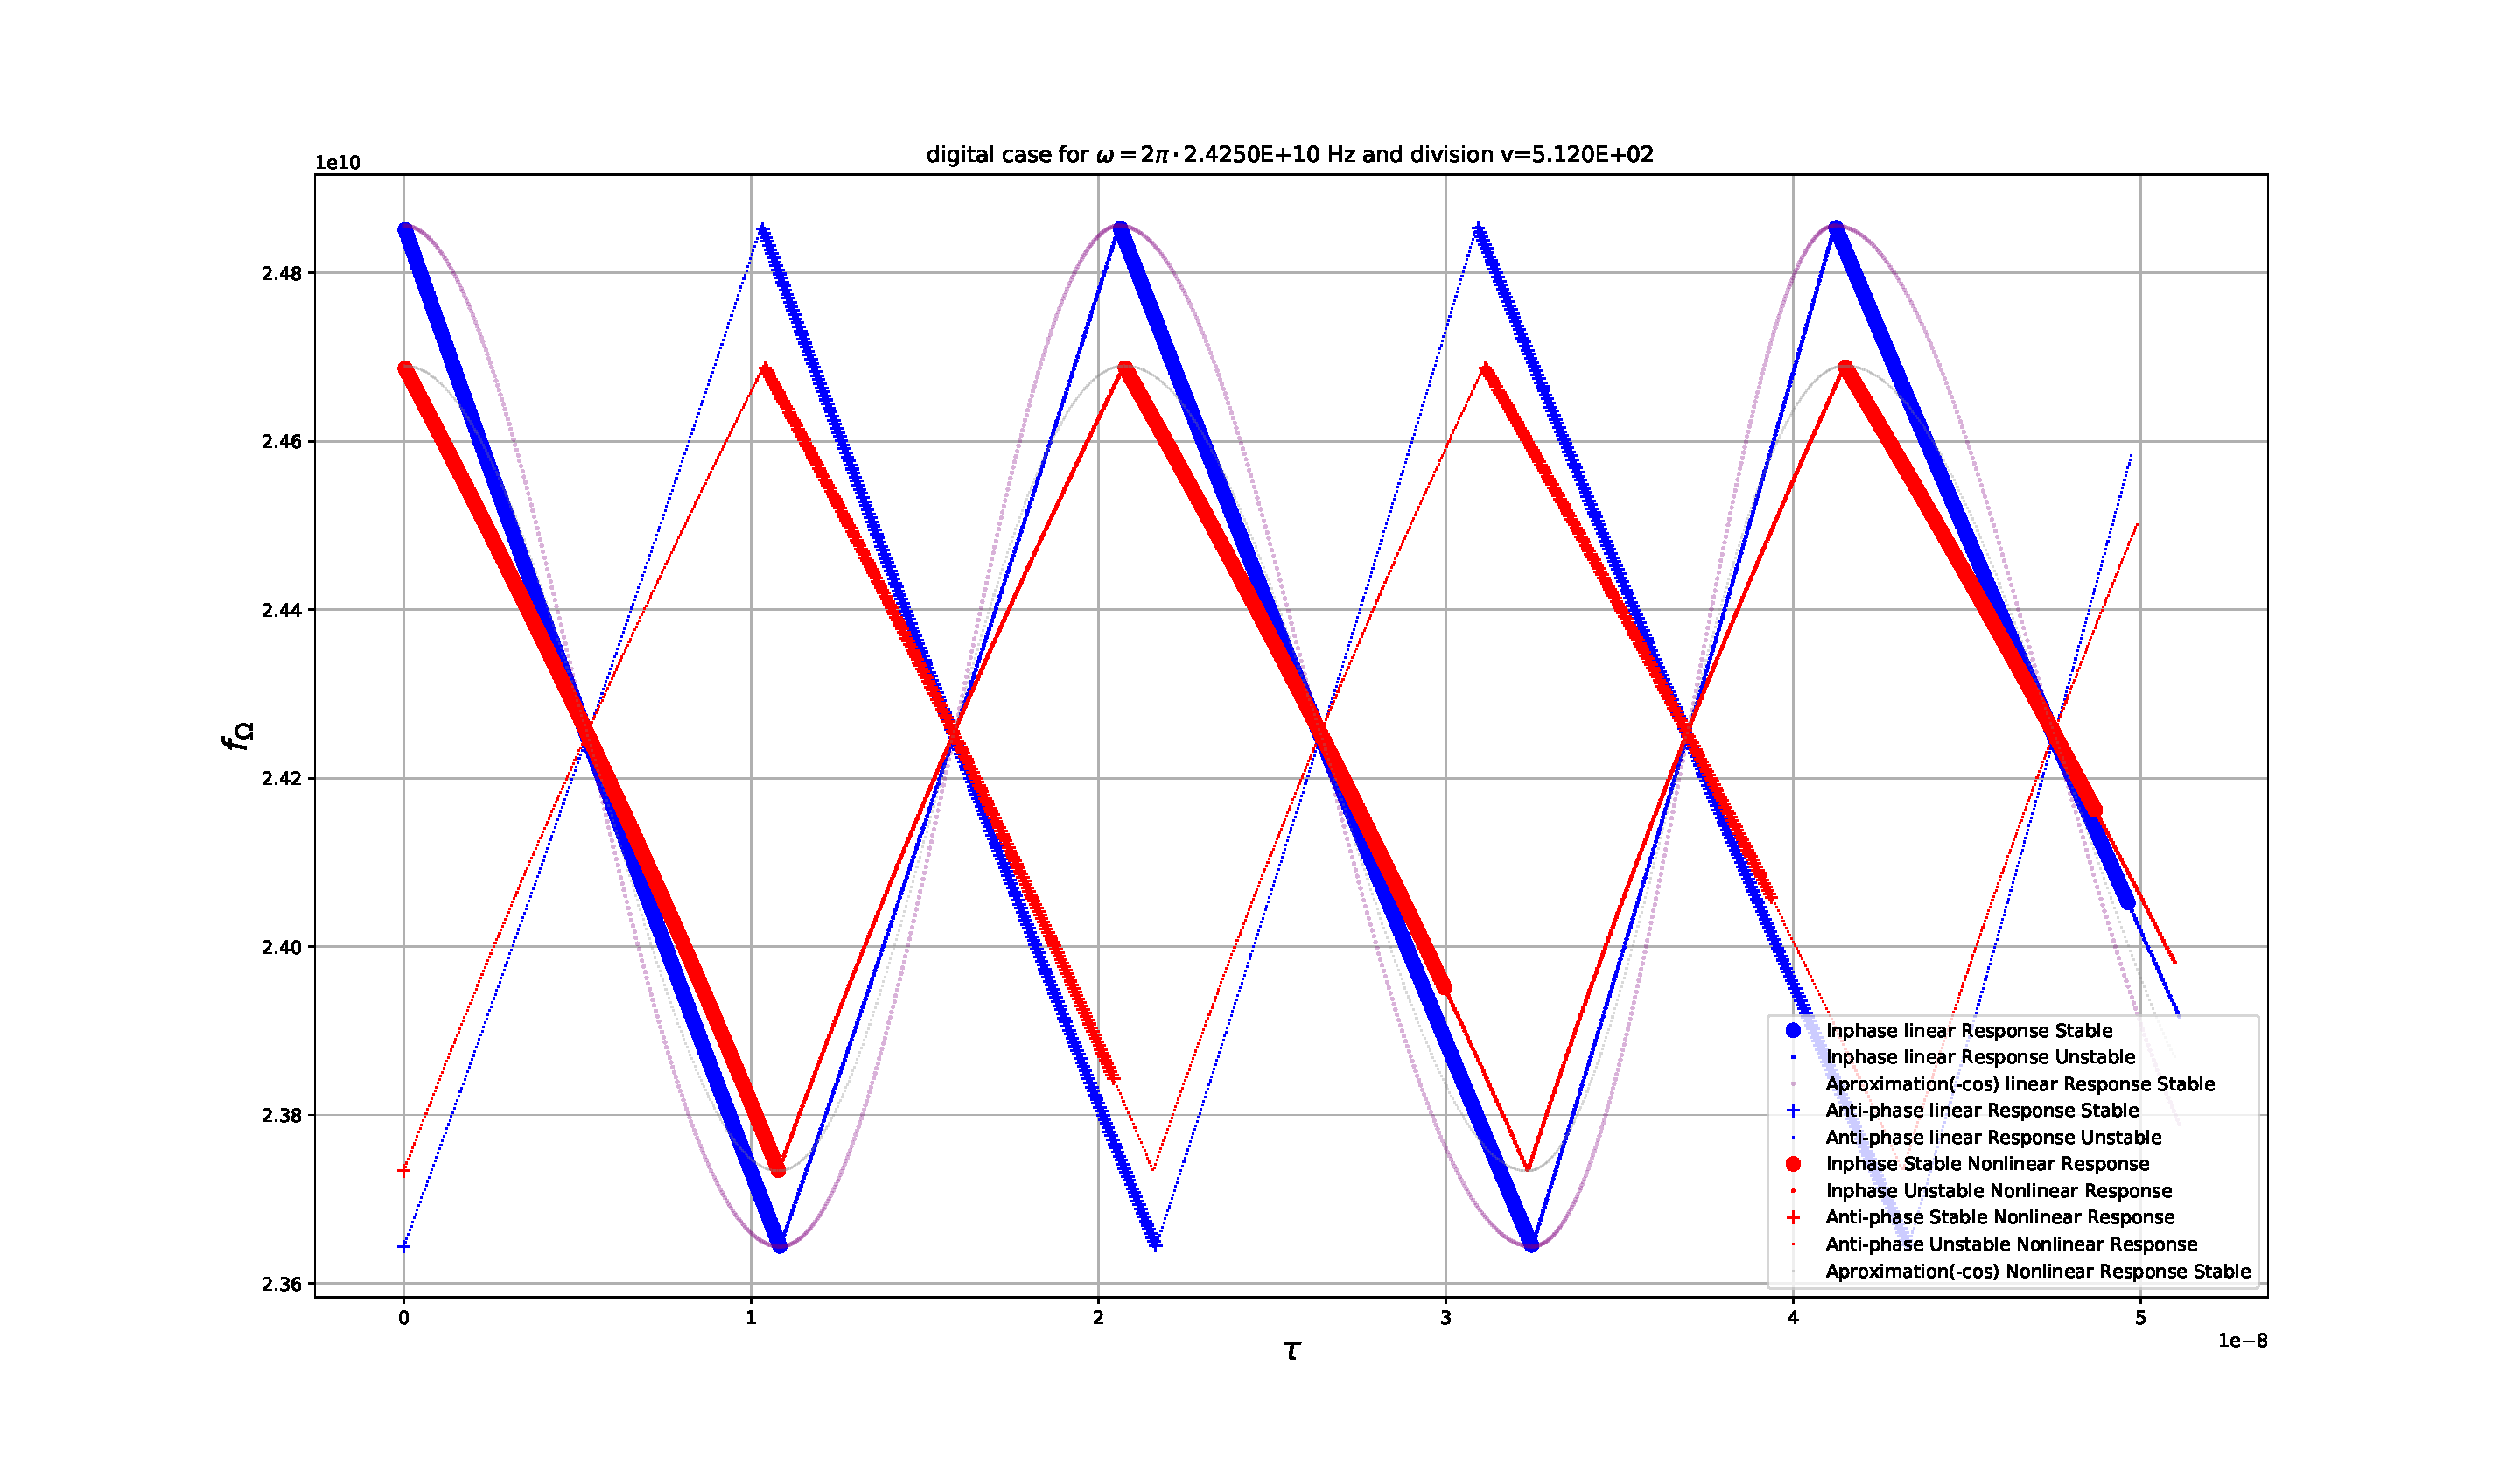
\includegraphics[width=17cm]{Omega_tau_3rdGen_linear_vs_Nonlinear_Freq_Response_pic1.pdf}	
	\caption{ }
	\label{fig:1}


\end{figure}

 In Fig.~(\ref{fig:1}) we plot the frequency of synchronized states, i.e., inphase and antiphase as a function of the delay. 
 %
 The blue marks refer to the model with the linear function of frequency response and the red to the model with the nonlinear function. 
 %
 The inphase synchronized states are presented with dots while the antiphase synchronized states with crosses. 
 %
 Larger sized markers denote stable synchronized states.

\begin{figure}[!h]
	\centering
	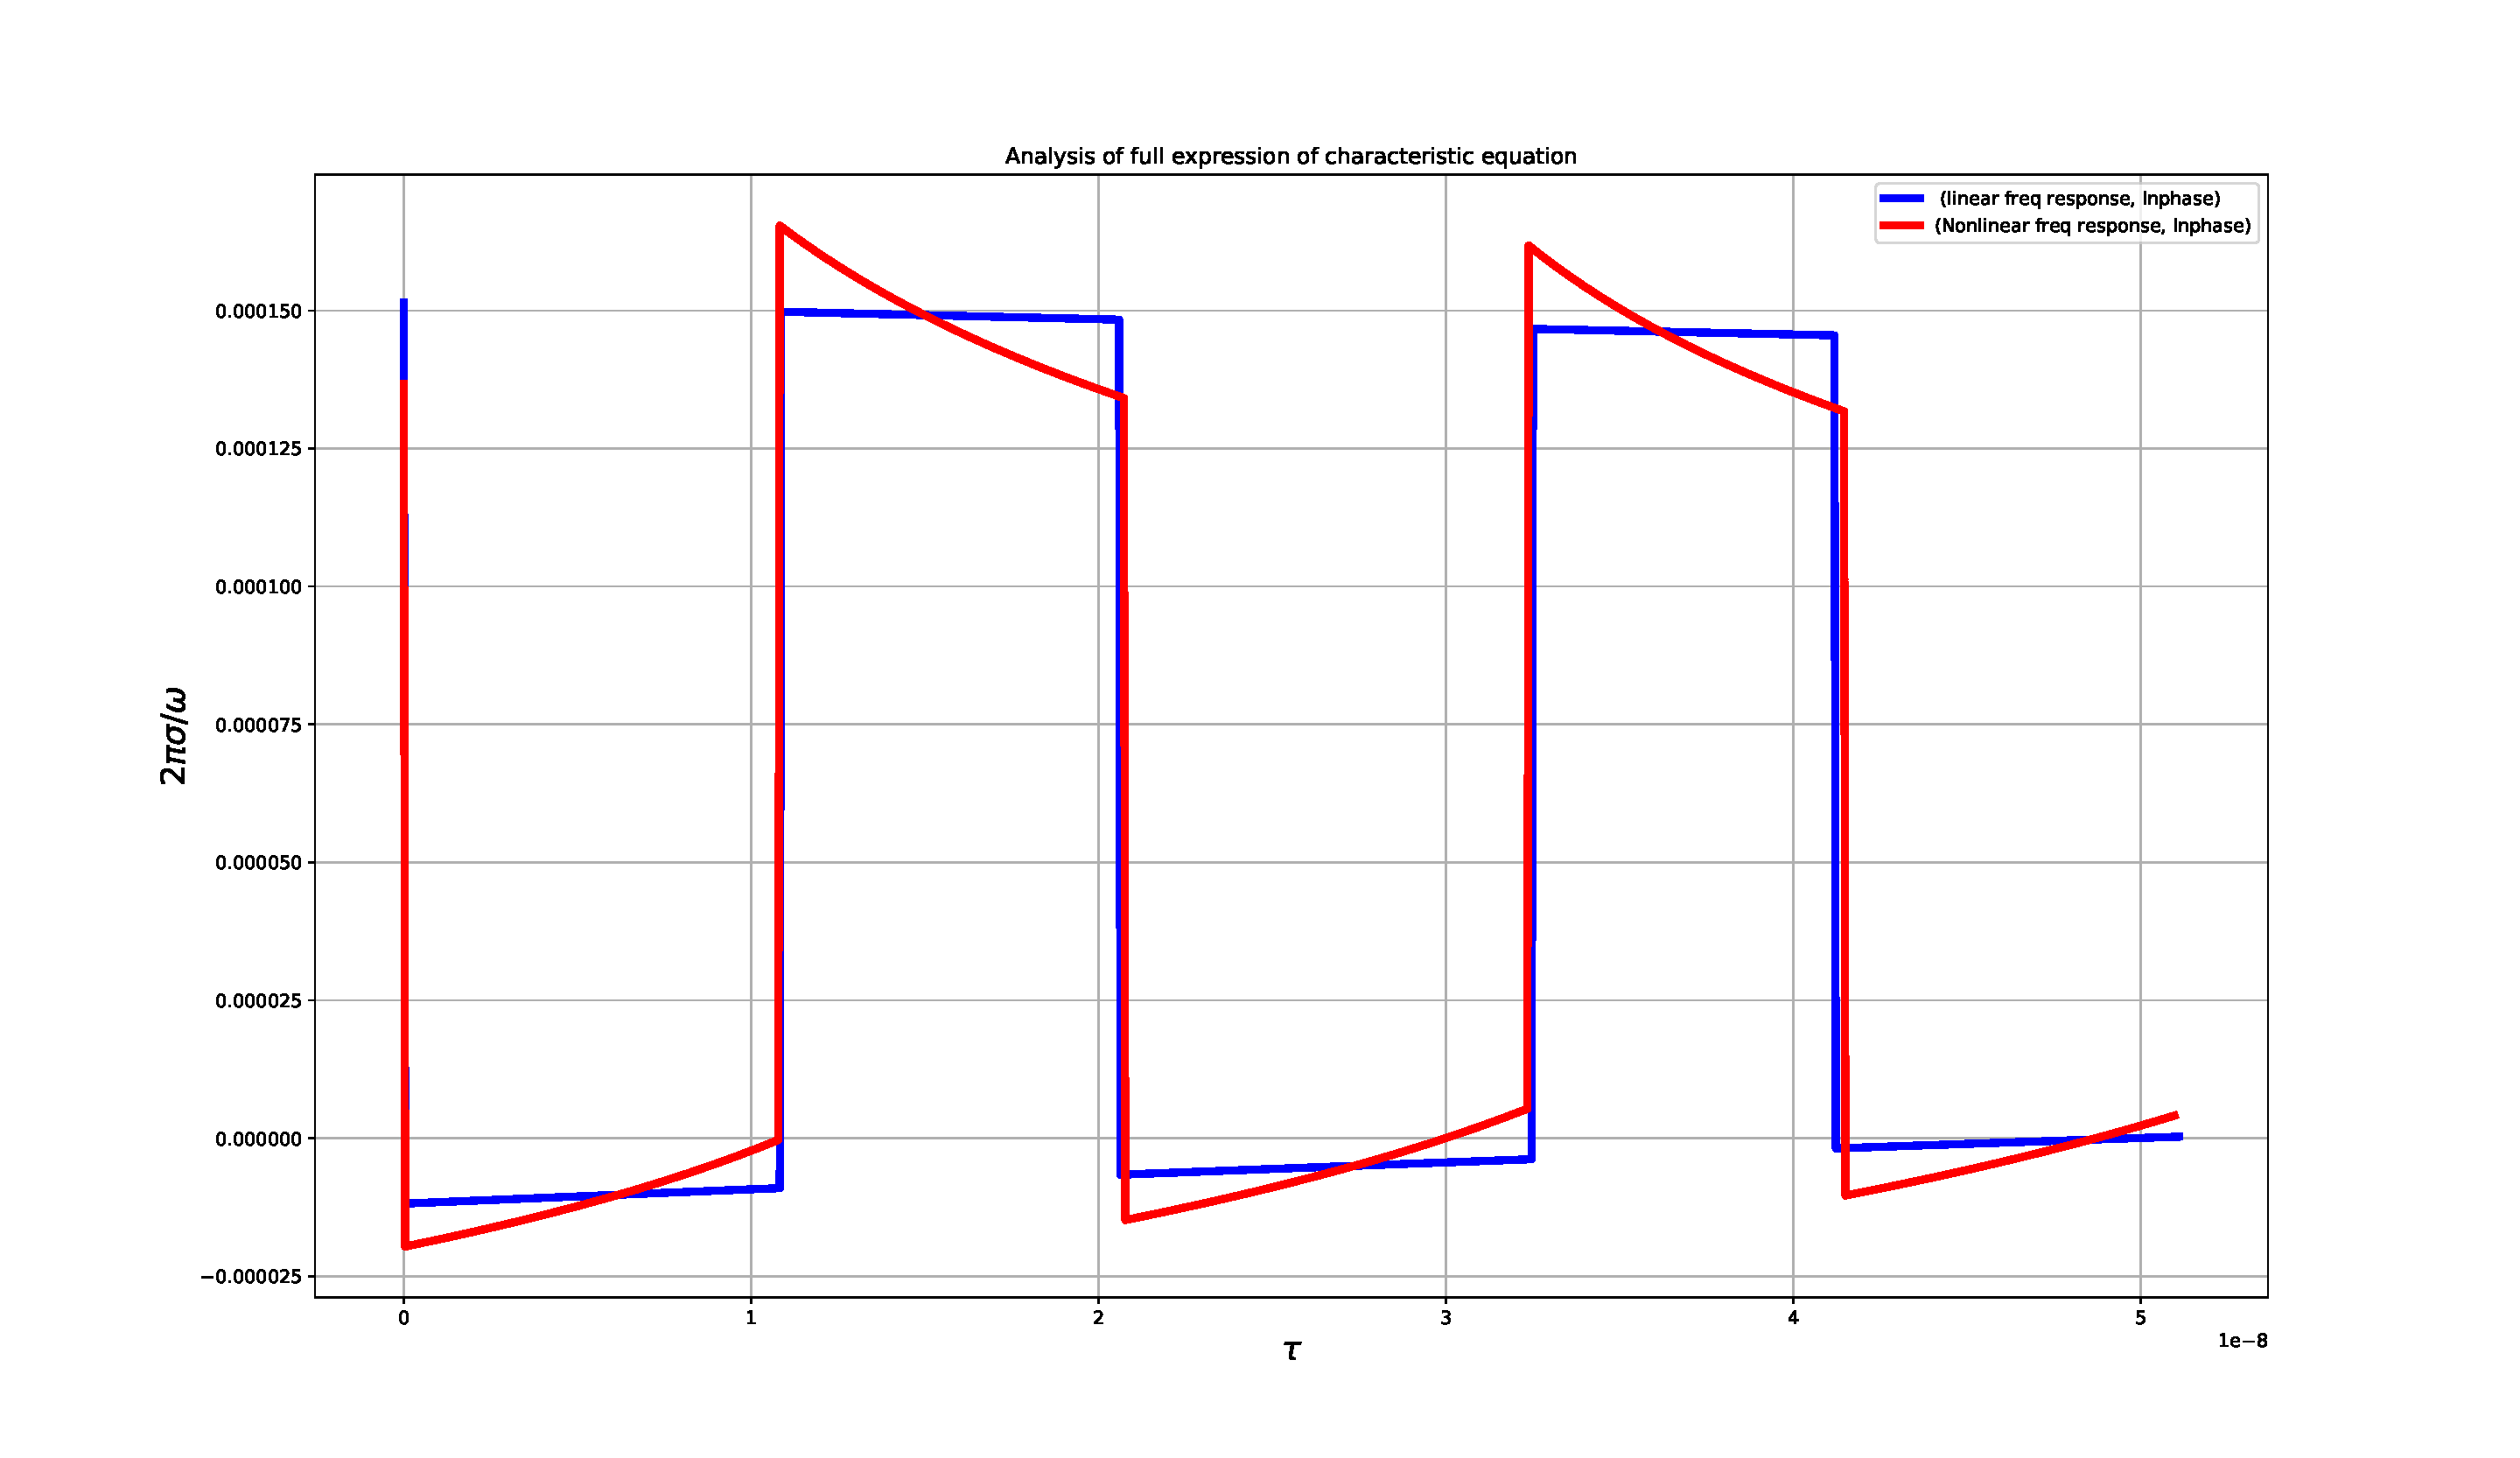
\includegraphics[width=17cm,height=8cm]{Sigma_tau_3rdGen_linear_vs_Nonlinear_Freq_Response_pic1.pdf}	
	\caption{ }
	\label{fig:2}
\end{figure}


In Fig.~(\ref{fig:2}) we plot the perturbation decay rate, $\sigma$, for both models as a function of the delay. 
%
We find that both models have the same $\sigma$ for frequencies close to the intrinsic frequency of the PLL. 
%
The perturbation decay rate for the nonlinear VCO response is different from that for the linear response approach.
%
In this particular case the nonlinearity of the VCO response leads to an asymmetric perturbation decay-rate about the intrinsic frequency of the PLL.
%
This means that the nonlinearity of the VCO affects the stability of the synchronized states. 
%
So the perturbation decay of a state with a frequency higher than the intrinsic frequency of the PLL is faster than that with a frequency that is smaller then the intrinsic PLL frequency. 
%
This means that synchronized states with frequencies smaller than the intrinsic PLL frequency decay perturbations more slowly then those obtained assuming a linear VCO response.


\end{document}
